% Session 3 -- chiral versus helical edge states, and what protects each.
% Placement: sec. "Quantum spin Hall insulators", after the Kramers paragraph.
% Rendered by figures/blender/s03f06_helical.py, labels in figures/overlays/s03f06_helical.tex.
\begin{aqmfigure}{fig:s03:helical}{Schematic edge dispersions for the two topological classes of
Section 3.8. The grey slabs are the bulk bands, and the branches that cross the bulk gap are the
edge states, plotted as a function of the momentum along the edge. (a) A Chern insulator has a
single branch per edge. At any energy in the gap there is one state and it moves in one direction,
so a scatterer has no state to send it back into. (b) A quantum spin Hall insulator has two
branches, one for each spin, drawn in a warm and a cold color, which propagate in opposite
directions on the \emph{same} edge, and this is what \textbf{helical} means. The total Chern number
vanishes, but the spin Chern number does not (3.9). (c) The crossing is not protected because the
two spin sectors are separately conserved. It is protected by Kramers' theorem, since the crossing
is at a time-reversal-invariant momentum, where a twofold degeneracy is guaranteed for spin-$1/2$
electrons for any perturbation that respects time reversal. Disorder that preserves time reversal
can therefore deform the branches but cannot gap them. Only a perturbation that breaks time reversal
opens the gap $\Delta$ in (c), and then the protection is lost.}
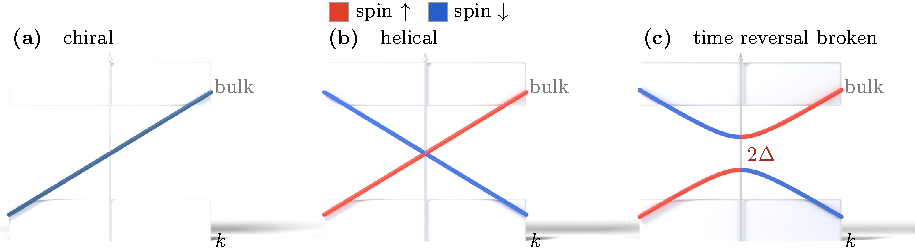
\includegraphics{figures/pdf/s03f06_helical.pdf}
\end{aqmfigure}
